% Q3 M0 figure/table insertion snippet; this file is not included by main.tex.
\begin{figure}[htbp]
  \centering
  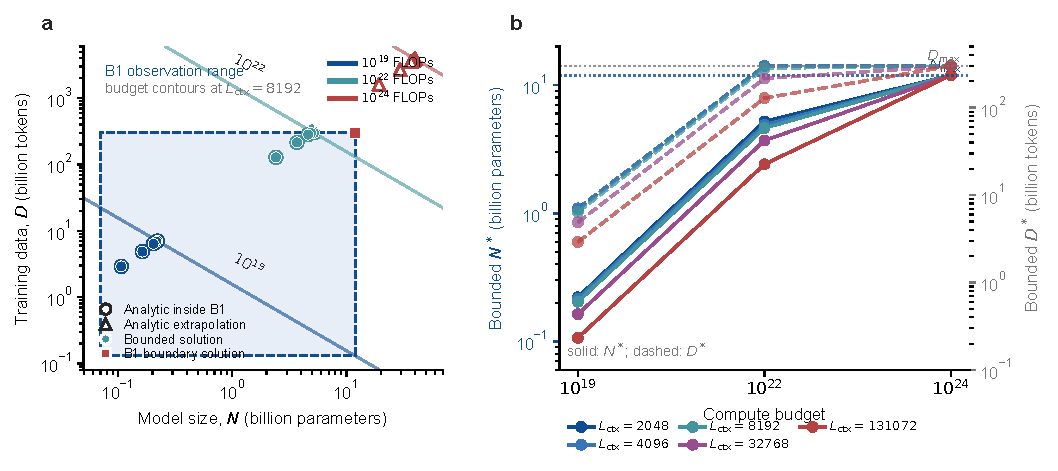
\includegraphics[width=\textwidth]{figures/q3-nd-baseline-nature-v1/fig_q3_m0_nd_frontier_nature_v1.pdf}
  \caption{M0 在 B1/Pythia 条件基线下的 $N$--$D$ 预算前沿。面板 (a) 给出 B1 观测范围、
  $L_{\mathrm{ctx}}=8192$ 时的等预算双曲线，以及解析放松点和 B1 范围内的有界解；
  三角形表示超出 B1 观测范围的解析外推点，方形表示触及 B1 边界的有界解。
  面板 (b) 给出五个观测上下文长度下的有界 $N^*$ 和 $D^*$ 随预算变化的条件前沿，
  水平虚线表示 B1 的 $N_{\max}$ 和 $D_{\max}$。全部 15 个场景直接来自运行
  \texttt{q3-nd-baseline-20260925-r01}；解析外推点和支持域内有界点按不同角色分别呈现。}
  \label{fig:q3-m0-nd-frontier}
\end{figure}

% Generated directly from q3-nd-baseline-20260925-r01/tables/q3_nd_baseline_scenarios.csv
\begin{table}[htbp]
  \centering
  \caption{M0 支持域内点与解析外推点的资源配置情景对比。}
  \label{tab:q3-m0-nd-scenarios}
  \scriptsize
  \begin{tabular}{r r c r c r l l}
    \toprule
    $C$ (FLOPs) & $L_{\rm ctx}$ & $(N,D)_{\rm relaxed}$ & $L_{\rm relaxed}$ & $(N,D)_{\rm bounded}$ & $L_{\rm bounded}$ & 状态 & 解析点角色 \\
    \midrule
$10^{19}$ & 2048 & (0.221, 7.050) & 2.9989 & (0.221, 7.050) & 2.9989 & B1范围内 & 域内解析点 \\
$10^{19}$ & 4096 & (0.215, 6.814) & 3.0114 & (0.215, 6.814) & 3.0114 & B1范围内 & 域内解析点 \\
$10^{19}$ & 8192 & (0.204, 6.403) & 3.0347 & (0.204, 6.403) & 3.0347 & B1范围内 & 域内解析点 \\
$10^{19}$ & 32768 & (0.163, 4.876) & 3.1412 & (0.163, 4.876) & 3.1412 & B1范围内 & 域内解析点 \\
$10^{19}$ & 131072 & (0.107, 2.908) & 3.3672 & (0.107, 2.908) & 3.3672 & B1范围内 & 域内解析点 \\
$10^{22}$ & 2048 & (5.007, 311.605) & 2.1432 & (5.202, 299.893) & 2.1432 & B1范围内 & 外推解析点 \\
$10^{22}$ & 4096 & (4.869, 301.196) & 2.1475 & (4.890, 299.893) & 2.1475 & B1范围内 & 外推解析点 \\
$10^{22}$ & 8192 & (4.626, 283.026) & 2.1556 & (4.626, 283.026) & 2.1556 & B1范围内 & 域内解析点 \\
$10^{22}$ & 32768 & (3.696, 215.518) & 2.1925 & (3.696, 215.518) & 2.1925 & B1范围内 & 域内解析点 \\
$10^{22}$ & 131072 & (2.415, 128.529) & 2.2707 & (2.415, 128.529) & 2.2707 & B1范围内 & 域内解析点 \\
$10^{24}$ & 2048 & (40.051, 3895.469) & 1.9134 & (11.966, 299.893) & 2.0934 & 边界约束 & 外推解析点 \\
$10^{24}$ & 4096 & (38.946, 3765.342) & 1.9155 & (11.966, 299.893) & 2.0934 & 边界约束 & 外推解析点 \\
$10^{24}$ & 8192 & (37.001, 3538.192) & 1.9195 & (11.966, 299.893) & 2.0934 & 边界约束 & 外推解析点 \\
$10^{24}$ & 32768 & (29.566, 2694.255) & 1.9377 & (11.966, 299.893) & 2.0934 & 边界约束 & 外推解析点 \\
$10^{24}$ & 131072 & (19.319, 1606.781) & 1.9763 & (11.966, 299.893) & 2.0934 & 边界约束 & 外推解析点 \\
    \bottomrule
  \end{tabular}
  \begin{flushleft}
  \footnotesize
  注：解析点由放松后的预算约束得到；当其超出 B1 观测范围时，标记为外推解析点。
  有界点在 B1 观测范围内求解，并保留边界状态。两类 Loss 分别对应各自的数学情景。
  \end{flushleft}
\end{table}

